\textit{EasyReporting} is a class\footnote{\url{https://en.wikipedia.org/wiki/Class_(computer_programming)}} builded with the intention of helping developers to integrating a reproducible research layer inside their software products.

In such a way, thanks to a minimal additional effort of the developer, the end user has available an \textit{rmarkdown} file within all the source code generated during the analysis, divided into \glspl{cc} ready for the compilation.

Once manually edited with comments and descriptions the file can be compiled to produce an enriched document within input data, source code and output results.

A so final document can be attached to the publication of the analysis as supplementary material, helping the interested community to entirely reproduce the computational part of work.

\subsubsection{General Description and Initialization}

The class has to be seen as a representation of the \textit{rmarkdown} file (\textit{report}), indeed it has been provided of a list of attributes describing the characteristics of the \textit{report}, which will be inserted in the header of the file.

The class methods are not only for the attributes manipulations, but also for adding \glspl{cc} to the \textit{report}.
 

Before of using it, \textit{easyReporting} requires to be initializated with the \lstinline!new! command, passing as mandatory arguments the \textit{path} and the name of the file as \lstinline!filenamepath! and a title as \lstinline!mainTitle!.
Additionally, an \lstinline!author! and the \lstinline!documentType! can be specified.

When initializing, the class automatically creates the \textit{report} with the entire specified folder tree, setting up the header of it and declaring the general options for the \textit{rmarkdown} file.
If \textit{rmarkdown} personal options (see figure \ref{fig:knitropts}) are required, before creating an instance of the class, it is possible to use the \lstinline!makeOptionsList! function, and then assigning the output to the \lstinline!optionsList! argument of the class \lstinline!constructor!.

\begin{figure}[H]
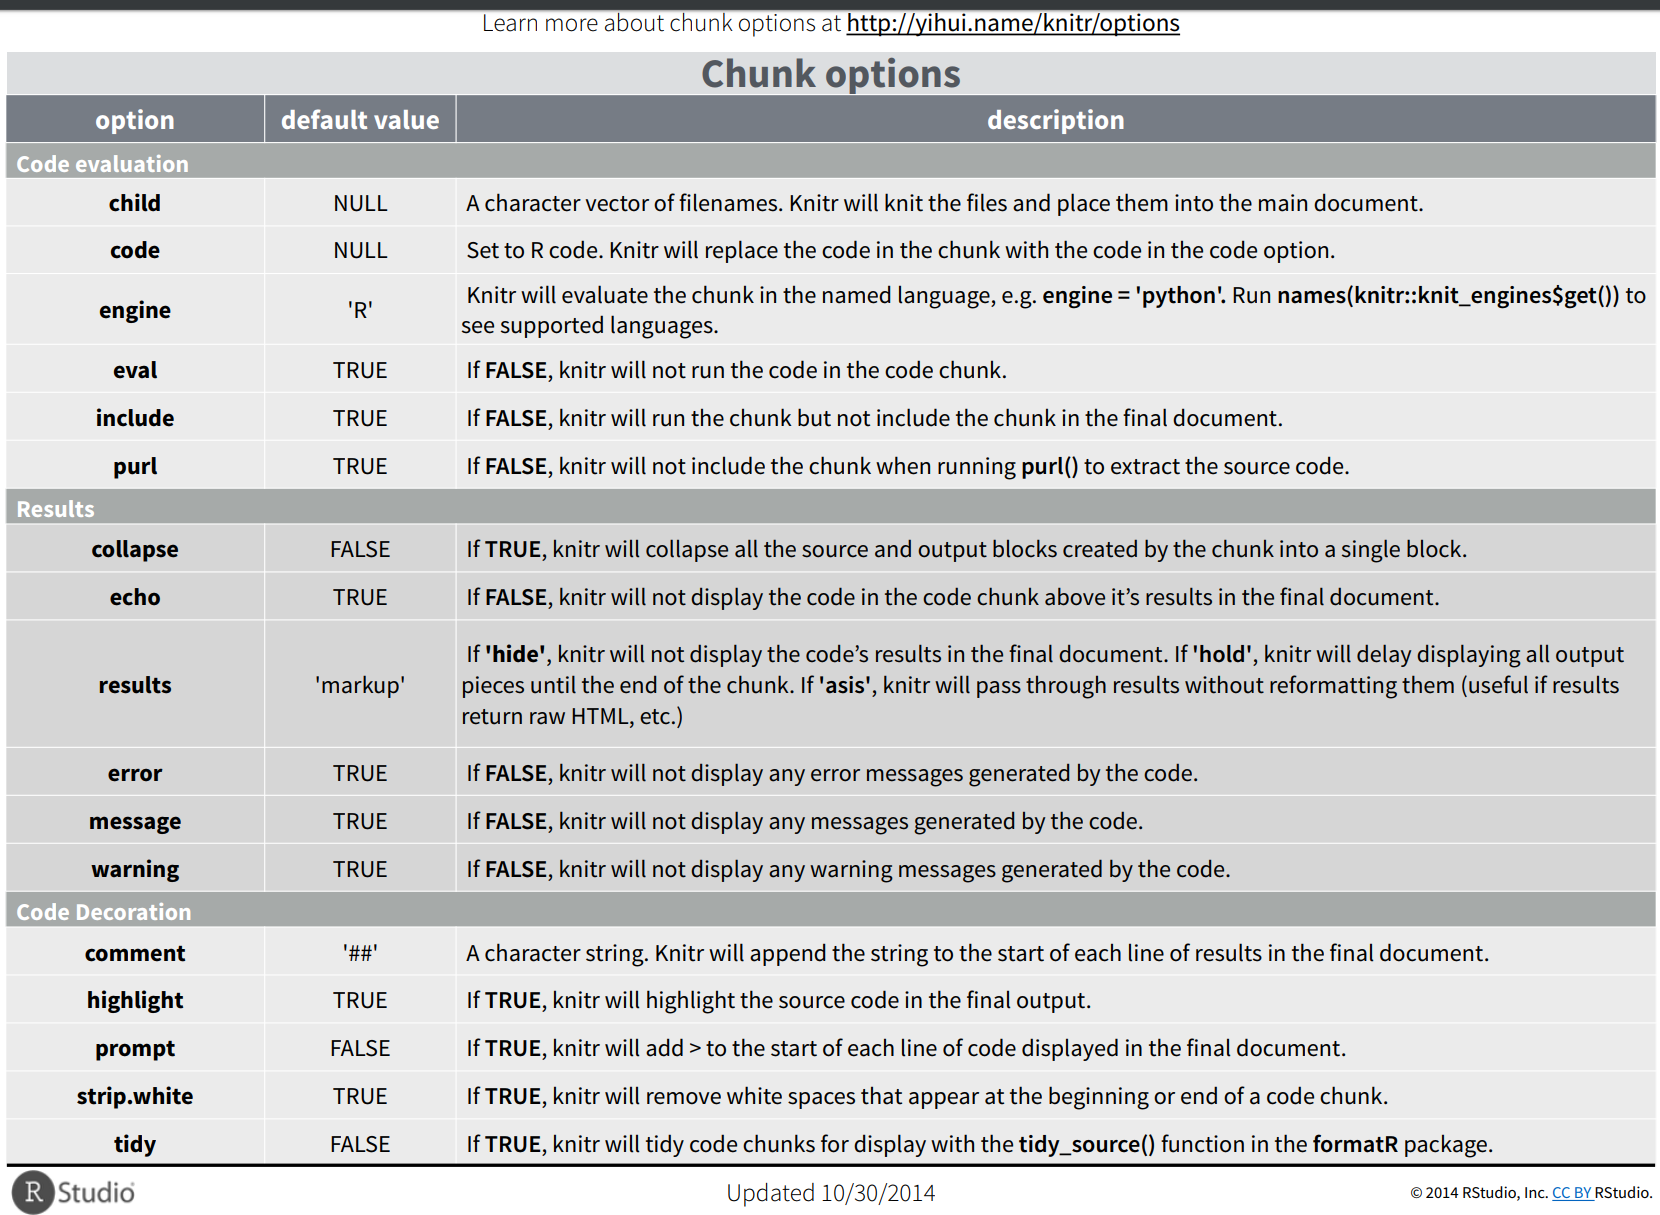
\includegraphics[width=\textwidth,height=\textheight,keepaspectratio]{img/rr/knitropts.png}
\caption[knitr options]{}
\label{fig:knitropts}
\centering
\end{figure}


\subsubsection{Class Methods}

The class is provided of several methods for \textit{rmarkdown} \gls{cc} construction.

Once an \textit{easyReporting} instance is available, with its \lstinline!mkdTitle! is possible to insert six levels of titles, by setting the parameters \lstinline!title! and \lstinline!level!.
It is also possible to add natural language comments with \lstinline!mkdGeneralMsg!.

When working with \glspl{cc}, two main possibilities are available.
The first one gives the possibility to construct a \gls{cc} as additional steps, by using first the \lstinline!mkdCodeChunkSt!, then adding variable assignment and/or function calling with \lstinline!mkdVariableAssignment! or \lstinline!mkdGeneralMsg!, and finally closing the \gls{cc} with \lstinline!mkdCodeChunkEnd!.

In particular, when starting a \gls{cc} with \lstinline!mkdCodeChunkSt!, it is possible to assign a specific \lstinline!optionList! and/or a \lstinline!source.files.list! to be added to that \gls{cc}.

The second way gives the possibility to create an entire \gls{cc} just with \lstinline!mkdCodeChunkComplete! and assigning the entire function call as a \lstinline!message!.
This way is really useful with function calls, where inside a function a simple recursive call with parameters assignment can be done as single \lstinline!message!.


\subsubsection{Usage Example}
Here we report a script where a fast illustration of the package is reported.
%
%\lstset{language=R,
%    basicstyle=\small\ttfamily,
%    numbers=left,
%	stepnumber=1,
%%	numbersep=5pt,
%%    stringstyle=\color{},
%%    otherkeywords={0,1,2,3,4,5,6,7,8,9},
%%    morekeywords={TRUE,FALSE},
%%    deletekeywords={data,frame,length,as,character},
%    keywordstyle=\color{blue},
%    commentstyle=\color{teal},
%   	backgroundcolor=\color{white},
%}

\begin{lstlisting}
## creating report file with default options on global document
rd <- easyreporting$new(filenamepath="./project_report", title="example_report", author=c("Dario Righelli"))

rd$mkdTitle("First Level Title")

rd$mkdGeneralMsg("Here I'm writing a simple paragraph useful to describe my code chunk")

## leaving the default options to the code chunk
rd$mkdCodeChunkSt()
## adding a variable assignement
variable <- 1
rd$mkdVariableAssignment("variable", "variable", show=TRUE)
rd$mkdCodeChunkEnd()

## or i can create my own options for the chunk
optList <- maketOptionsList(includeFlag=TRUE)
rd$mkdCodeChunkSt(optionsList=optList)
rd$mkdCodeChunkEnd()

## moreover I can add a list of files to source in che code chunk
rd$mkdCodeChunkSt(optionsList=optList, source.files.list=c("R/cachingFunctions.R", "R/cachingFunctions.R"))
rd$mkdCodeChunkEnd()


rd$mkdCodeChunkComplete(message="a <- 1\nb <- 2\nc <- a+b\n print(c)")


## otherwhise i can make a direct call with all the code chunk and the code as message


rd$compile()


\end{lstlisting}
 
